\subsection{Performance comparison with iZ3 and MathSat}\label{performance_euf}

This section discusses a benchmark for interpolant generation
for the EUF theory.
which it will allows us to test 
our implementation and constrast the execution with 
other interpolant generation
algorithms from Z3 and MathSat.

\subsubsection{Benchmark description}

The bench mark uses the following parameters:

\begin{itemize}
  \item[] $i$ stands for the number of constants
  \item[] $j$ stands for the number of function symbols
    with arity between 2 and 3
  \item[] $k$ stands for limit for random terms to consider
    in the problem
  \item[] $n$ stands for the equations/disequations in the
    A-part
\end{itemize}

The benchmark generates a pair of two unsatisfiable formulas
in the EUF language from a fixed theory with the following parameters:

\begin{equation*}
  S = \{ c_1, \dots, c_i, f_1, \dots, f_j \}
\end{equation*}

where $i, j$ are random integer numbers. Using the $S$, we
enumerate the grounded terms $G$ in $S$ and assign a natural 
number to each number denoting its position in the enumeration.

We generate $n$ random equations/disequations from the signature $S$ 
such that this
collection of formulas is consistent for the $A-part$ of
the input problem. 
The latter is implemented using a $z3: :solver$ to ensure 
this condition.
The equations/disequations are of the form

\begin{equation*}
  position(k_1, S) = position(k_2, S) \text{ , or } position(k_1, S) \neq position(k_2, S) 
\end{equation*}

where $position(k, S)$ denotes the $k^{th}$ element in $G$. The 
integers $k_1, k_2$ are choosen uniformly at random from a
distribution of integer values $\{0, \dots, k\}$, 
where $k$ is a parameter of the benchmark.

Next we randomly generate a second set of consistent 
equations/disequations (B-Part) until the $A-part$ and the
$B-part$ are inconsistent using a second $z3: :solver$.

We designed this problem because it is not trivial to 
compute a  uniform/interpolant due to randomness of the
problem. This problem was executed $100$ times
with parameters (i=10, j=5, k=100, n = 10) and 
(i=20, j=10, k=100, n = 40)
using a computer desktop
equipped with an Intel i7-9700 @ 4.70 GHz processor 
and 16Gb of RAM. 

The following graph reports the time needed
by our implementation, iZ3, and the interpolation 
generation algorithm from Mathsat. 
It is well known that both iZ3 and Mathsat does not
compute uniform interpolants. Regardless, the benchmark
was used with the purpose to compare their execution time
on normal interpolants.

The time was
measured using a bash script which takes the difference
of the output produced by the UNIX utility $date +`\%s.\%N'$ 
at the beginning and at the end of the execution of the 
tested algorithms.

\begin{figure}
  \centering
  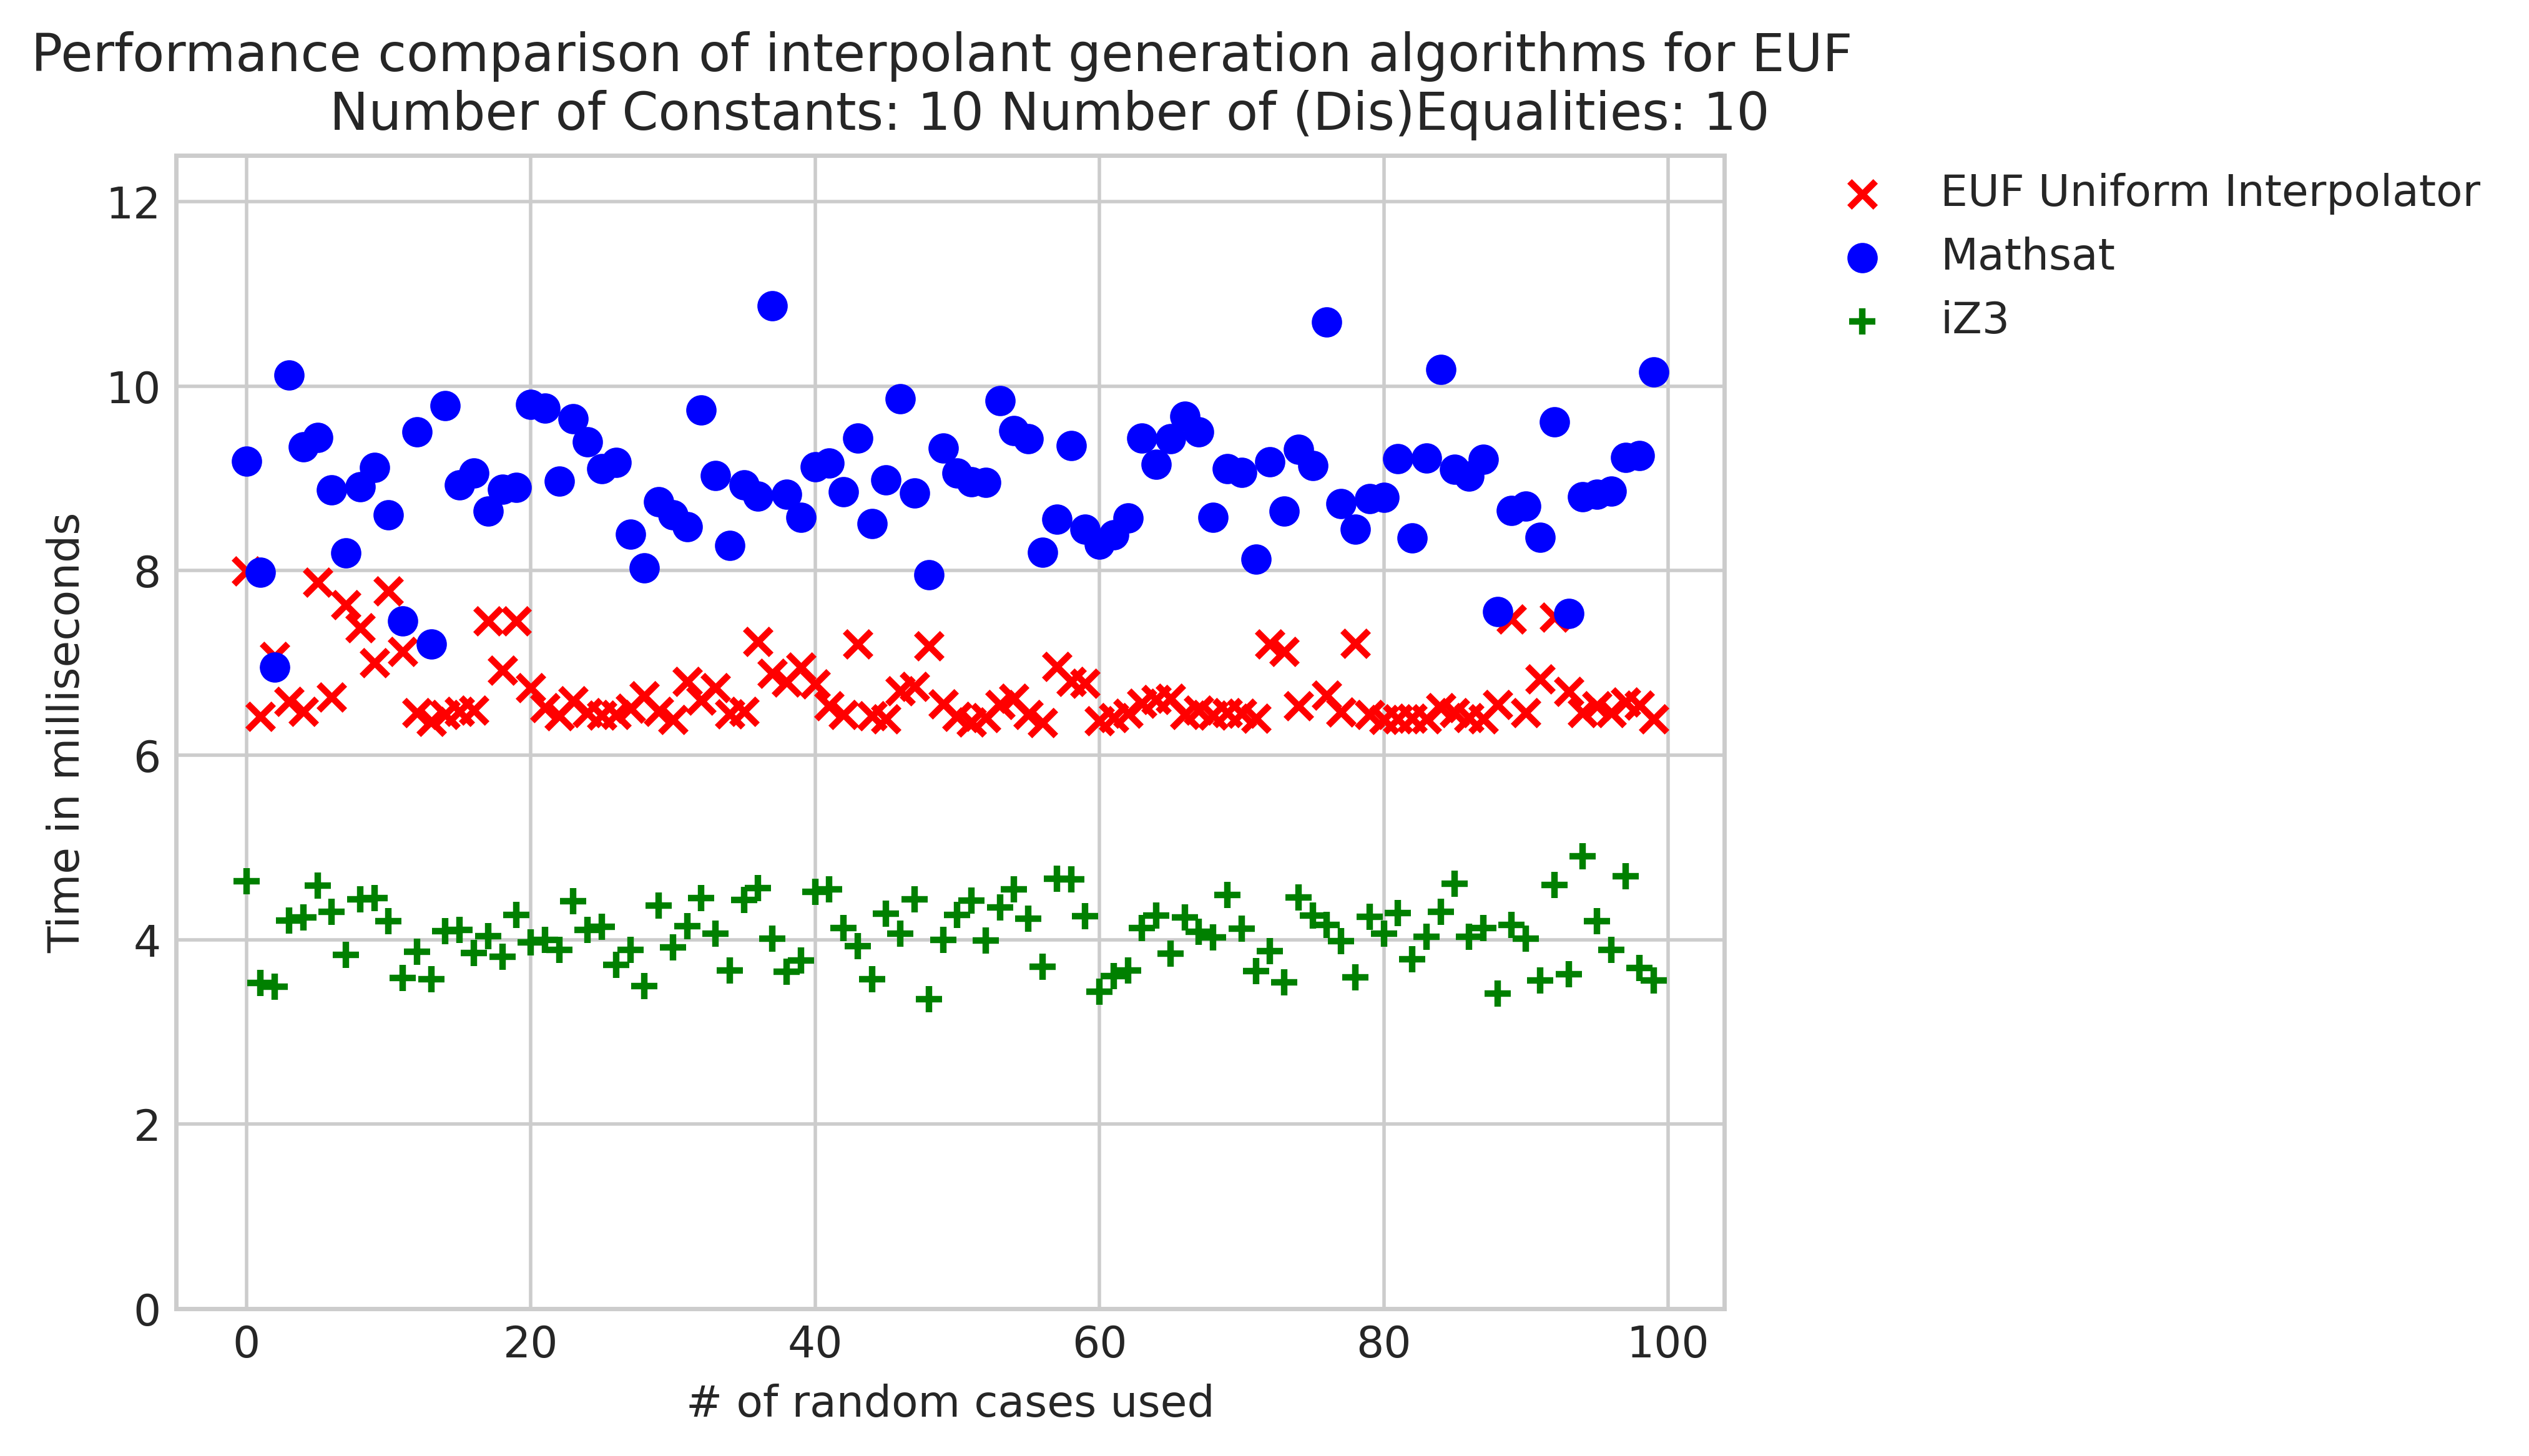
\includegraphics[scale=0.9]{figures/eufi_performance_graph_10_5_3_10_100}
  \caption{Performance comparison graph of EUF interpolant generation
  algorithms for paramatrized problem from section \ref{performance_euf}} 
  \label{performance_graph_euf}
\end{figure}

\begin{figure}
  \centering
  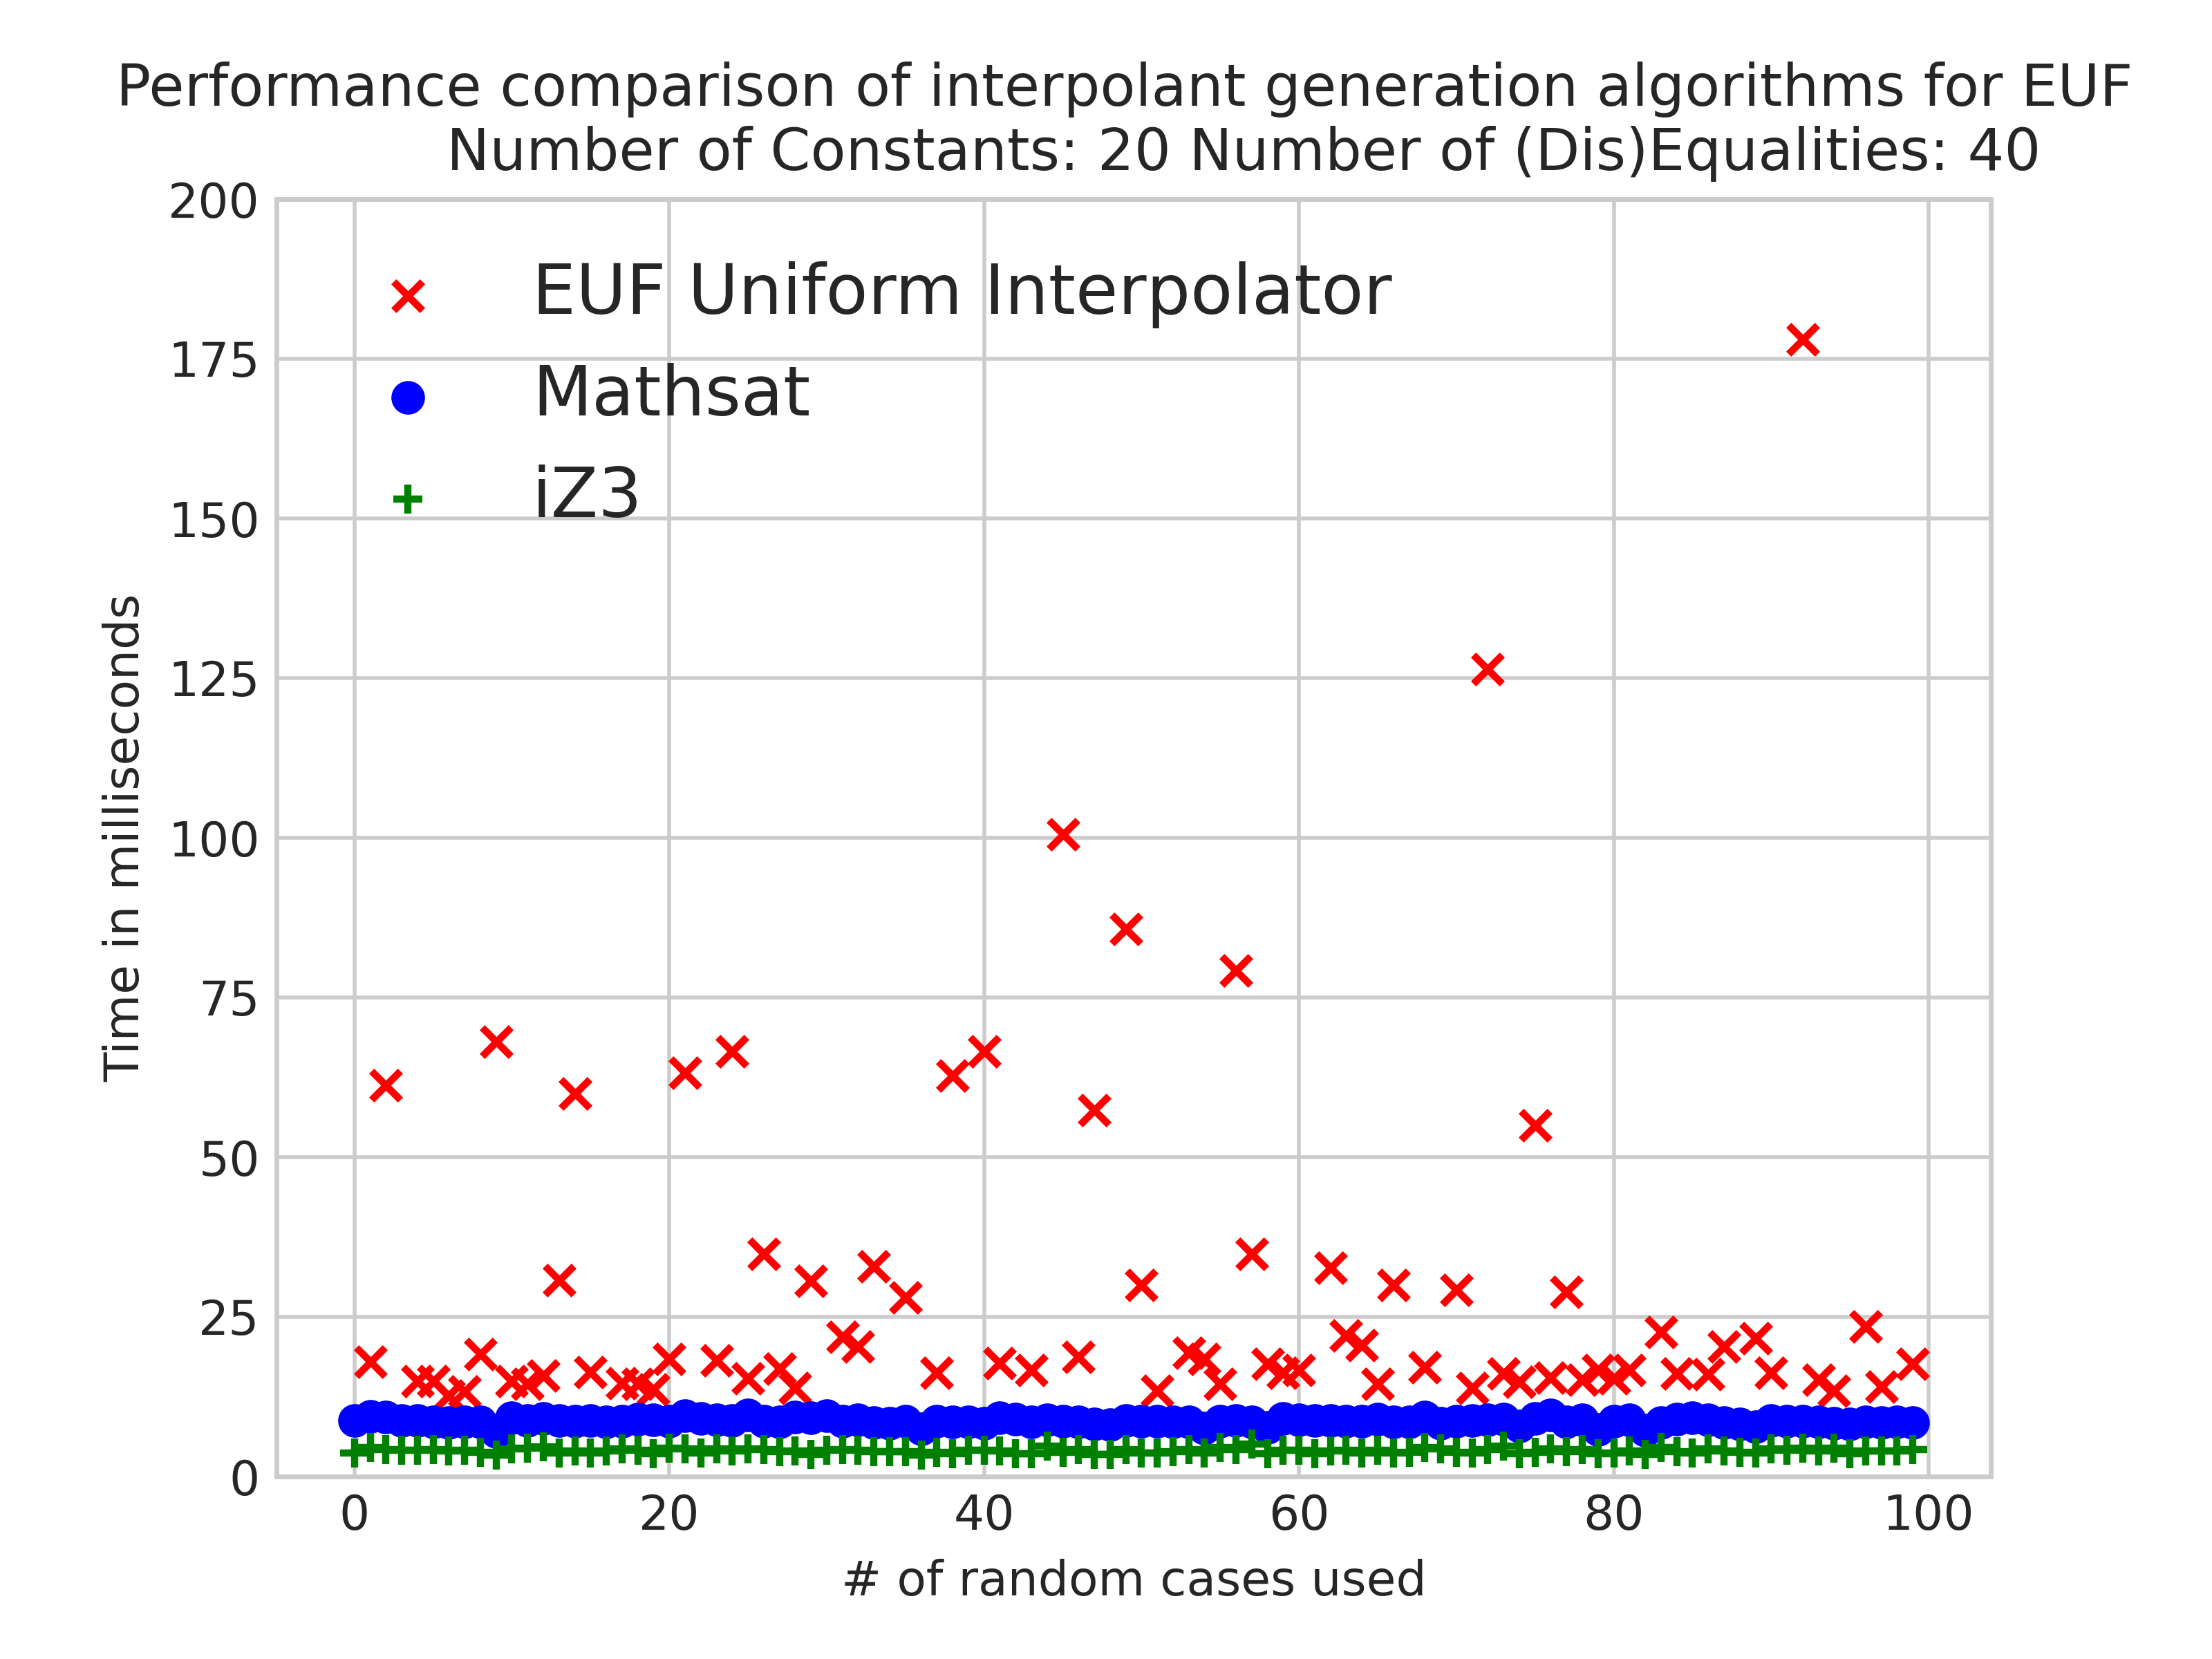
\includegraphics[scale=0.9]{figures/eufi_performance_graph_20_10_3_40_100}
  \caption{Performance comparison graph of EUF interpolant generation
  algorithms for paramatrized problem from section \ref{performance_euf}} 
  \label{performance_graph_euf}
\end{figure}

%%% Local Variables:
%%% mode: latex
%%% TeX-master: "main"
%%% End:
